\documentclass[10pt]{article}
\usepackage{graphicx} % Required for inserting images
\usepackage{geometry}
\usepackage{hyperref}
\usepackage{tabularx}

\geometry{a4paper,left=20mm,right=20mm,top=20mm}
\graphicspath{{src/assets}}

\title{Relazione Progetto di Tecnologie Web}
\author{
    \textbf{2076430}\\ Gusella Manuel \and
    \textbf{2075541}\\ Marcon Giulia \and
    \textbf{2082849}\\ Perozzo Andrea \and
    \textbf{2075515}\\ Tutino Giuseppe
}
\date{A.A. 2024/25}

\begin{document}

\begin{figure}
    \centering
    
\includegraphics[width=0.5\linewidth]{logo.png}
\end{figure}
\maketitle
\renewcommand{\arraystretch}{2}
\begin{tabular}{|>{\centering\arraybackslash}m{7cm}|>{\centering\arraybackslash}m{8cm}|}
    \hline
     Link Sito Web & \url{} \\
     \hline
     E-mail referente del gruppo & manuel.gusella@studenti.unipd.it \\
    \hline
\end{tabular}
\newpage
\tableofcontents
\newpage

\section{Introduzione}
\subsection{Abstract}
"Doflamingo" è un marketplace digitale che contiene delle opere uniche sotto forma di NFT pubblicate direttamente dall'associazione.
Un Non-fungible token (NFT) rappresenta l'atto di proprietà e certificato di autenticità di un bene unico, in questo caso un'opera digitale. \\
Tutti i visitatori hanno la possibilità di visionare le opere e creare il proprio account digitale.\\
Gli utenti registrati possono comprare le opere, se non già possedute da qualcun'altro, attraverso una valuta digitale chiamata Ethereum (ETH). Eventualmente l'utente può decidere di vendere le opere che possiede ad altri utenti.\\ 
Inoltre gli utenti registrati possono recensire le opere dando un voto da \textbf{1 a 5 stelle}, inserendo opzionalmente anche un commento al riguardo.\\


\subsection{Analisi}
\subsubsection{Analisi del Target}
L'utenza principale sarà composta da persone appassionate agli NFT e alla loro compra-vendita. La maggioranza degli utenti non avrà un'idea precisa di ciò che vuole e per questo verrà aiutata nell'esplorazione.\\
Per impedire l'esclusione di alcune categorie si è pensato di fornire strumenti per aiutare nella ricerca degli NFT.\\
Utilizzando la metafora della pesca:
\begin{itemize}
    \item \textbf{Tiro perfetto:} L'utente sà già il nome dell'opera che vuole e potrà cercarla facilmente tramite una barra di ricerca;
    \item \textbf{Trappola per aragoste:} Grazie alla suddivisione in categorie e poter applicare ulteriori filtri sulle opere l'utente può farsi un'idea degli NFT presenti nella piattaforma.
    \item \textbf{Pesca con la rete:} La struttura del sito è semplice, quindi permette agli utenti di esplorare il sito senza sovraccarico
    \item \textbf{Boa di segnalazione:} 
\end{itemize}
\subsubsection{Utenti}
Esistono 3 tipologie di utenti:
\begin{itemize}
    \item Utente non registrato, che può eseguire le seguenti azioni:
    \begin{itemize}
        \item Visualizzare il sito con le relative opere
        \item Registrare un proprio account
        \item Autenticarsi
        \item Ricerca delle opere
        \item Visualizzare i dettagli di un'opera con le relative recensioni
    \end{itemize}
    \item Utente registrato, che può eseguire le seguenti azioni:
    \begin{itemize}
        \item Comprare le opere
        \item Recensire le opere
        \item Visualizzare le opere che possiede
        \item Vendere le opere che possiede
    \end{itemize}
    \item Amministratore, che può eseguire le seguenti azioni:
    \begin{itemize}
        \item Gestire gli utenti
        \item Aggiungere opere
        \item Visualizzare le vendite
    \end{itemize}
\end{itemize}

\section{Progettazione logica del database}

\subsection{Descrizione schema relazionale}
\begin{itemize}
    \item \textbf{utente} (\underline{username}, password, email, isAdmin, saldo)
    \item \textbf{categoria} (\underline{nome}, descrizione)
    \item \textbf{iscrizione} (\underline{\textit{utente}, \textit{categoria}})
    \item \textbf{opera} (\underline{id}, path, nome, descrizione, prezzo, \textit{possessore})
    \item \textbf{acquisto} (\underline{\textit{utente}, \textit{opera}}, prezzo, data)
    \item \textbf{appartenenza} (\underline{\textit{categoria}, \textit{opera}})
    \item \textbf{recensione} (\underline{timestamp, \textit{utente}}, commento*, \textit{opera}, voto)
\end{itemize}
Il simbolo * indica che l'attributo può essere nullo.

\subsection{Vincoli di integrità referenziale }
\begin{itemize}
    \item iscrizione.utente → utente.username
    \item iscrizione.categoria → categoria.nome
    \item opera.possessore → utente.username
    \item acquisto.utente → utente.username
    \item acquisto.opera → opera.id
    \item appartenenza.categoria → categoria.nome
    \item appartenenza.opera → opera.id
    \item recensione.utente → utente.username
    \item recensione.opera → opera.id
\end{itemize}
\subsection{Schema E-R}
\begin{center}
    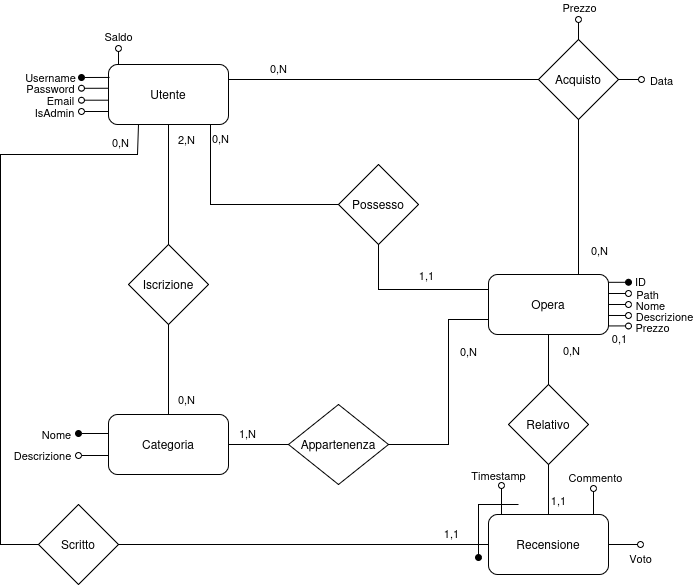
\includegraphics[width=0.6\linewidth]{schema_ristrutturato.png}
\end{center}

\section{Linguaggi}
\subsection{HTML}
Le pagine sono state create seguendo gli standard HTML5, dato che si presuppone che l'utente visiterà la pagina tramite browser più aggiornati.
\subsection{CSS}
Per rispettare la separazione tra struttura e presentazione si è deciso di utilizzare fogli di stile esterni.
\subsection{SQL}
Il sito web si appoggia su un database per le informazioni degli Utenti, delle opere, delle recensioni, degli acquisti e delle categorie.
\subsection{PHP} 
Per rispettare la separazione tra struttura e comportamento si è deciso di utilizzare script in PHP. Questi script vengono utilizzati per connettersi al database, visualizzare determinati NFT nelle pagine ed effettuare controlli di autenticazione.
\subsection{JavaScript}
JavaScript è stato utilizzato per gestire la visualizzazione dinamica dei filtri nella pagina e per implementare uno slider orizzontale nella galleria di contenuti.

\section{Progettazione}
Per la progettazione abbiamo utilizzato la strategia \textit{Mobile First}. Questo approccio permette di concentrarci sulla modalità di accesso principale per la maggioranza degli utenti, cioé quella da mobile. Ci siamo focalizzati soprattutto sul diminuire il numero di click/tap necessari per accedere alle varie sezioni del nostro sito.
\subsection{Struttura generale}
Il sito non ha una profondità elevata ed è composto da:
\begin{itemize}
\item \textbf{Home:} Visualizzata come landing page per accogliere l'utente che entra nel sito;
\item \textbf{NFT:} Pagina dedicata alla ricerca delle opere presenti nel sito;
\item \textbf{Singolo NFT:} Pagina dedicata ad un singolo NFT. Vengono visualizzate tutte le informazioni dell'opera, il prezzo per poterla acquistare e le recensioni degli utenti dell'opera. 
\item \textbf{Chi Siamo:} Pagina di presentazione dei componenti del gruppo in cui è presente anche un FAQ per le domande più frequenti tra gli utenti;
\item \textbf{Registrati:} L'utente utilizzerà questa pagina per registrarsi nella piattaforma;
\item \textbf{Login:} L'utente utilizzerà questa pagina per accedere al proprio profilo;
\item \textbf{Profilo:} Pagina che contiene le informazioni personali dell'utente, le opere in suo possesso e le recensioni che ha realizzato.
\end{itemize}

\subsection{Header e Navbar}
Nell'Header è sempre presente il logo per poter definire l'identità del sito.\\
Inoltre sarà sempre presente una navbar che permetterà, grazie al numero non elevato di sezioni, all'utente di vedere subito in quale pagine può navigare senza l'utilizzo di tap aggiuntivi, cosa che servirebbe se avessimo usato un menù ad hamburger. Per evitare link circolari il link della pagina corrente viene rimosso e reso riconoscibile rispetto agli altri.\\
Saranno presenti due navbar:
\begin{itemize}
\item Una per l'utente non autenticato dove saranno presenti le sezioni \textbf{Home}, \textbf{NFT}, \textbf{Chi Siamo}, \textbf{Registrati}, \textbf{Accedi};
\item Una per l'utente autenticato dove saranno presenti le sezioni \textbf{Home}, \textbf{NFT}, \textbf{Chi Siamo}, \textbf{Profilo}, \textbf{Log out}. 
\end{itemize}

\subsection{Breadcrumb}
All'interno di ogni pagina sarà presente la Breadcrumb per informare l'utente dove si trova e per ridurre il disorientamento. Viene rispettato il livello di profondità, mostrando le pagine padri precedenti alla pagina corrente. Per evitare link circolari la pagina corrente non viene resa cliccabile.

\subsection{Contenuto}

\section{Implementazione}
\subsection{Front-End}
\subsection{Back-End}

\section{Organizzazione del lavoro}
\subsection{Gusella Manuel}
\subsection{Marcon Giulia}
\subsection{Perozzo Andrea}
\subsection{Tutino Giuseppe}

\end{document}

%  dove l'arte del futuro incontra la tecnologia blockchain..
